\chapter{Introduction}
What and where is dark matter? For a question so central to cosmology and particle physics, the prospects for finding an answer do not at first glance seem promising. As with so many things in physics, we should not by all rights be able to answer the question, nature having hidden itself away in the dark recesses of the universe. But dark matter is all around us and we merely need a window through which to view it. In this work, I will discuss strategies for the direct detection of dark matter: how they offer us a window - however murky - into the dark universe; how they are faced with myriad  uncertainties; and how those uncertainties can be overcome to help us to understand more about what dark matter is and how it is distributed in our tiny patch of the universe.

The question `\textit{What is dark matter?}' is perhaps best answered by reviewing the current evidence for its existence. Evidence for dark matter is found on scales from the Milky Way up to the cosmological horizon, with a range of observations which cannot be adequately explained with the observed constituents of the universe. Dark matter is an invisible component introduced to reconcile these observations with the known laws of physics - most importantly, General Relativity. Beyond this general definition, there are a wide range of particle physics candidates which may play the role of dark matter. These typically derive from theories of physics beyond the Standard Model, meaning that the study of the properties of dark matter can shed light on theories of high energy physics. Many of these proposed dark matter candidates have weak but non-zero interactions with particles of the Standard Model, leading to several avenues through which it is hoped the non-gravitational detection of dark matter may soon be achieved.

In this chapter, we summarise the evidence in support of the dark matter paradigm, including constraints from precision cosmology. We then describe some of the broad classes into which particle dark matter candidates can be categorised, as well as describing a few specific candidates in more detail. Finally, we discuss current progress and constraints from direct and indirect searches for particle dark matter.

\section{Evidence for dark matter}

Dark matter is a key component of the \LCDM paradigm of modern cosmology. In this framework, the energy density of the universe today is dominated by the constant and uniform contribution of the vacuum, $\Lambda$, also referred to as Dark Energy. This contribution exerts a negative pressure and drives the accelerating expansion of the universe which was the subject of the 2011 Nobel Prize in Physics \cite{Riess:1998, Perlmutter:1999}. However, the formation of structure in the early universe is driven by the clustering of an inert, slow moving and as yet undetected matter component \cite{Kolb:1990}: Cold Dark Matter. In \LCDM cosmology, baryonic matter makes up a much smaller fraction of the energy density of the universe. Cosmological experiments allow us to precisely determine the contributions of these various components (see e.\ g.\  WMAP \cite{Hinshaw:2013}, BOOMERanG \cite{MacTavish:2005}, BOSS \cite{Dawson:2013}, BICEP2 \cite{Ade:2014} and CFHTLenS \cite{Kitching:2014} to name just a few.)

A particularly sensitive probe for determining the dark matter contribution to the energy budget of the universe is the measurement of the temperature anisotropies of Cosmic Microwave Background (CMB) photons. These contain an imprint of the acoustic oscillations of the baryon-photon fluid during the era of recombination. The scale of these oscillations is sensitive to the size of the gravitational potential generated in the early universe by dark matter. \note{This is shite and needs fixing, am I talking about BAOs or what?} The recent Planck experiment \cite{PlanckI:2013} measured the angular power spectrum of these CMB temperature anisotropies. Figure~\ref{fig:intro:CMB} shows the results of these measurements, as well as the best fit 6-parameter \LCDM model. The contribution of the cosmological constant, the total matter component, and the separate baryonic and dark matter components to the total energy density of the universe is shown in Table~\ref{tab:intro:Planck}, constrained with an accuracy of less than 3\%. We are lead to the conclusion that $\sim$84\% of the matter content of the universe is in fact dark.

\note{Do more evidence - and less `problems' - maybe move the BBN stuff here?}

\todo{Read for details: arXiv:1404.5415}

\note{CFHTLENS: arXiv:1404.5469}

\begin{figure}[h]

  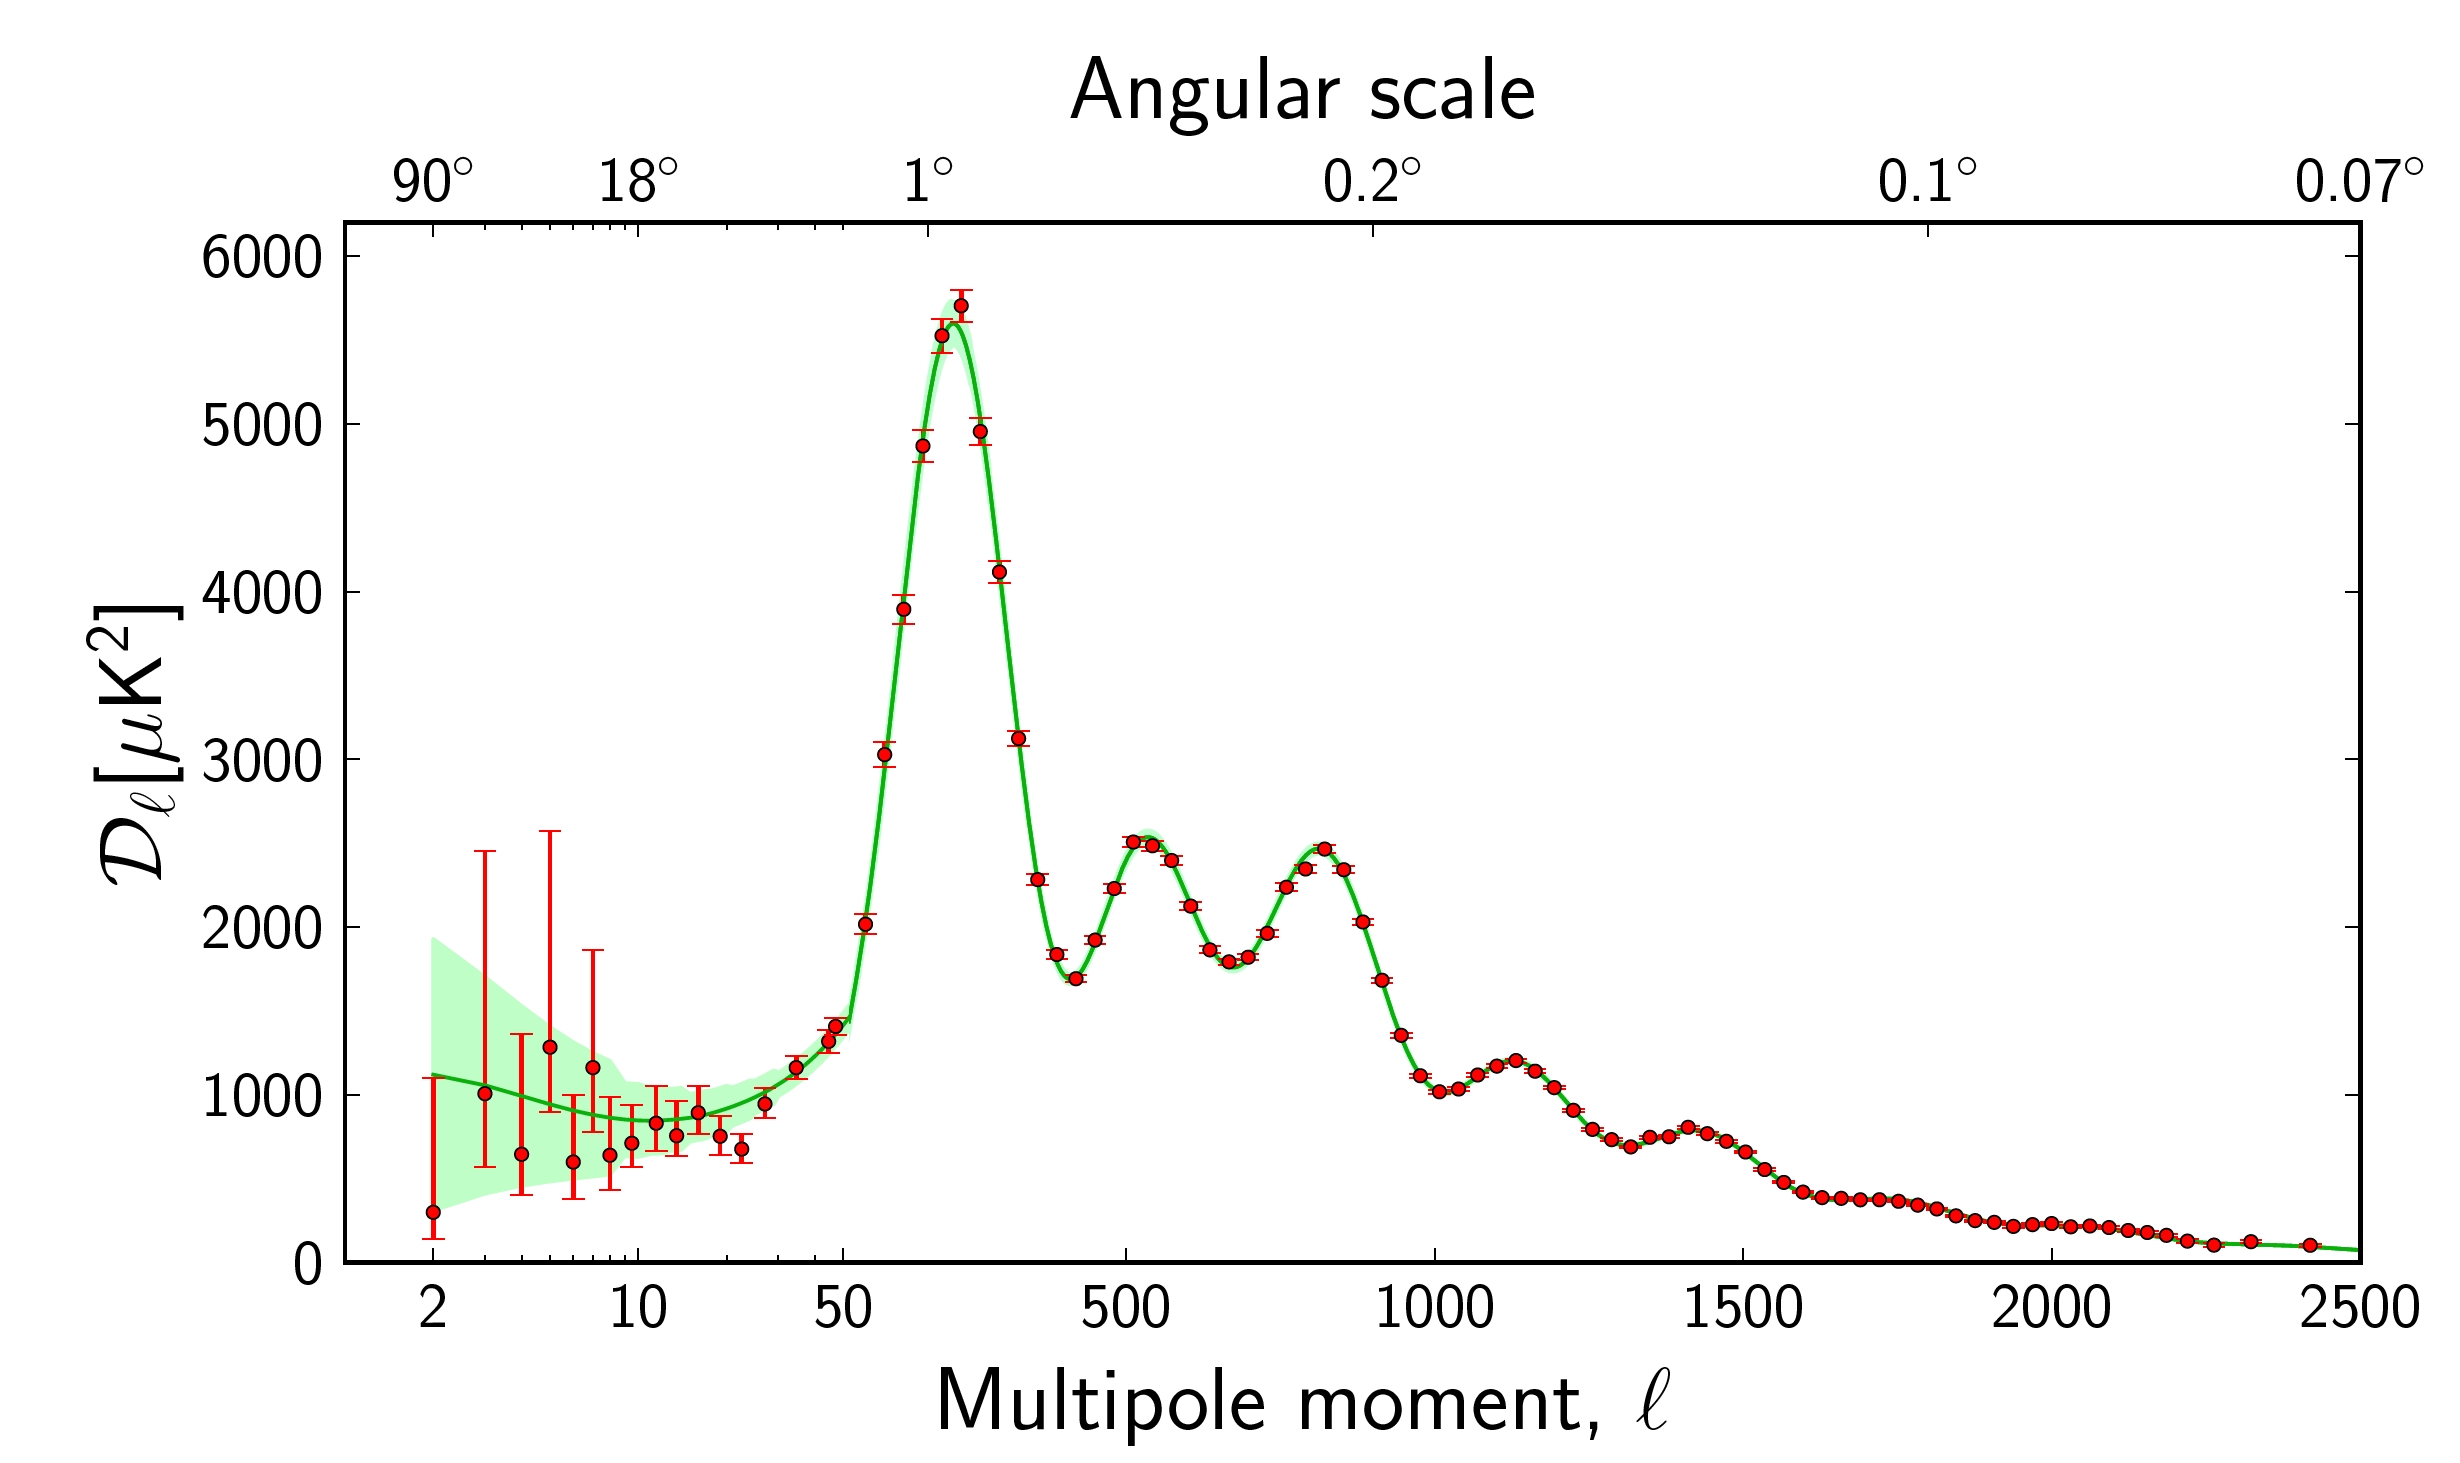
\includegraphics[width=\textwidth]{CMBanisotropies.jpg}
  \caption[CMB anisotropies measured by the Planck experiment]{CMB anisotropies. \note{Need actual caption}}
  \label{fig:intro:CMB}
\end{figure}


\begin{table}

  \begin{center}
	\begin{tabular}{cc}
        \hline\hline
        Parameter & 68\% limits \\
        \hline
        $\Omega_\Lambda$ & 0.686 $\pm$ 0.020 \\
        $\Omega_m h^2$ & 0.1423 $\pm$ 0.0029 \\
        $\Omega_b h^2$ & 0.02207 $\pm$ 0.00033 \\
        $\Omega_c h^2$ & 0.1196 $\pm$ 0.0031 \\
        \hline\hline
	\end{tabular}
  \end{center}
  \caption[Cosmological parameters obtained by the Planck Collaboration]{Energy density of the cosmological constant ($\Lambda$), total matter ($m$), and separate baryonic ($b$) and cold dark matter ($c$) components in units of the critical density \note{define...}, as obtained by the Planck Collaboration \cite{PlanckXVI:2013}. The Hubble parameter is defined as $H_0 = 100 \,\,h \, \textrm{km s}^{-1} \textrm{Mpc}^{-1}$.}
  \label{tab:intro:Planck}
\end{table}

However, the evidence for dark matter is not purely cosmological. In 1933, Zwicky measured the velocity dispersion of galaxies in the Coma cluster \cite{Zwicky:1933}. An application of the Virial Theorem indicated a gravitational mass in the cluster which was several hundred times bigger than that expected from the luminosity of the member galaxies. It is now known that some of this mass is in the form of hot ($\sim$1 million K), X-ray emitting intracluster gas \cite{Sanders:2013}. Nonetheless, a discrepancy remains; current estimates of the mass-to-light ratio of the Coma cluster give a value of roughly 150 times that of the Sun \cite{Fusco-Femiano:1994,Makino:1994}. However, the Coma cluster does not appear to be unusual. Measurements of the masses of a large number of galaxy clusters using gravitational lensing \cite{Okabe:2013}, X-ray observations \cite{Ettori:2013} and dynamical estimates \cite{Carlberg:1995} indicate that a significant fraction of a cluster's mass must be dark.

The validity of the \LCDM paradigm is also borne out in results from N-body simulations. These simulations track the evolution of structure in the universe by accounting for the dynamics and gravitational interactions \note{only Newtonian?} of a large number of particles starting from some initial conditions. These may be horizon-scale cosmological simulations, tracing the collapse of the initial density perturbations after decoupling (such as the the Millenium simulation \cite{Springel:2005}), or galaxy-scale simulations, tracing the formation and growth of a small number of galaxies starting from initial conditions at intermediate redshift (such as the Via Lactea \cite{Diemand:2006} and Aquarius \cite{Springel:2008} simulations).

\note{Maybe swap this paragraph with the next one - it makes more sense?} A variety of sophisticated computational techniques (such as smoothed particle hydrodynamics \cite{Stinson:2010}, adaptive mesh refinement \cite{Norman:1999} and moving mesh cosmology \cite{Springel:2010}) have been employed and refined to make such simulations computationally feasible and to allow higher and higher resolutions to be reached. In spite of this, computational limitations mean that the highest resolution simulations still use `particle' masses of the order of $10^5 M_{\odot}$ \cite{Pillepich:2014}, many orders of magnitude more massive than the $O$(GeV-TeV) particles expected to make up the universe's dark matter. \note{say more...}

Many N-body simulations are DM-only, simulating only the gravitational dynamics of collisionless particles. However, an increasing number are incorporating baryonic physics such as gas dynamics, as well as stellar evolution, chemical enrichment and a variety of feedback processes \note{Need some citations...}. Appropriately accounting for these factors is extremely complex and in some cases the strength of these processes is unknown and must be tuned in the simulations to match observations (see for example Ref.~\cite{Vogelsberger:2013}). \note{Mention some other problems - shock resolution etc.} Due in part to these difficulties, the impact of baryonic physics on the formation of galaxies and the properties of DM haloes is still uncertain (see for example Refs.~\cite{Martizzi:2012,Pillepich:2014}). I will revisit this topic - and its consequences for the direct detection of dark matter - in Chapter~\ref{ch:DirectDetection}.

In spite of these limitations, a consistent picture has emerged from a vast array of N-body simulations. The size distribution of gravitational structures found in the universe is well matched over a range of distance scales  with that obtained from N-body simulations \note{CITATION!}. In particular, the fact that DM is non-interacting means that it begins to collapse gravitationally earlier in cosmic time than baryonic matter. After decoupling, baryons then fall into the gravitational wells produced by the infalling DM structures. Without DM, the baryonic matter in the universe could not have had enough time to collapse to form the array of gravitationally bound structures we see today \cite{Kolb:1990}. \note{Coldness...}

N-body simulations also suggest that galaxies such as the Milky Way should be embedded in a large, approximately spherical dark matter halo. This is corroborated by observations of the rotation curves of spiral \note{just spirals?} galaxies. In particular, the circular velocity of stars in these galaxies is observed to be approximately constant out to large galactocentric distances \cite{Begeman:1991,Persic:1996}. This is shown schematically in Fig.~\ref{fig:intro:RotationCurves}. \note{Say something about gas, and 21cm emission (so that you can check the rotation beyond the luminous matter). [Optical edge]} The majority of the mass of the luminous disc is concentrated at small radii, suggesting that there should be a Keplerian decay of the circular velocity at large radii: $v \sim r^{-1/2}$. However, the inclusion of a non-luminous dark matter halo can reconcile this expectation with the observed flat rotation curves. The density profiles $\rho(r)$ required to provide a good fit to rotation curve data are consistent with those obtained from N-body simulations, such as the Navarro-Frenk-White profile \note{Is this really true? Cusp/Core problem?}

\begin{equation}
\label{eq:intro:NFW}
\rho(r) = \frac{\rho_0}{r/R_s(1 + r/R_s)^2}\,,
\end{equation}
which is described by the central density $\rho_0$ and a scale radius $R_s$. This provides a good cross-check between the results of N-body simulations, which span scales up to the cosmological, and galactic-scale observations of the local universe. The rotation curve of the Milky Way itself has also been studied \note{[cite Mattia and others self-consistent distribution guys]}, as well as the ultralocal distribution of dark matter near the Sun's position. An understanding of this distribution has significant implications for the study of dark matter detection and we defer a detailed discussion to Chapter~\ref{ch:DirectDetection}.

\begin{figure}[h]

  \centering
  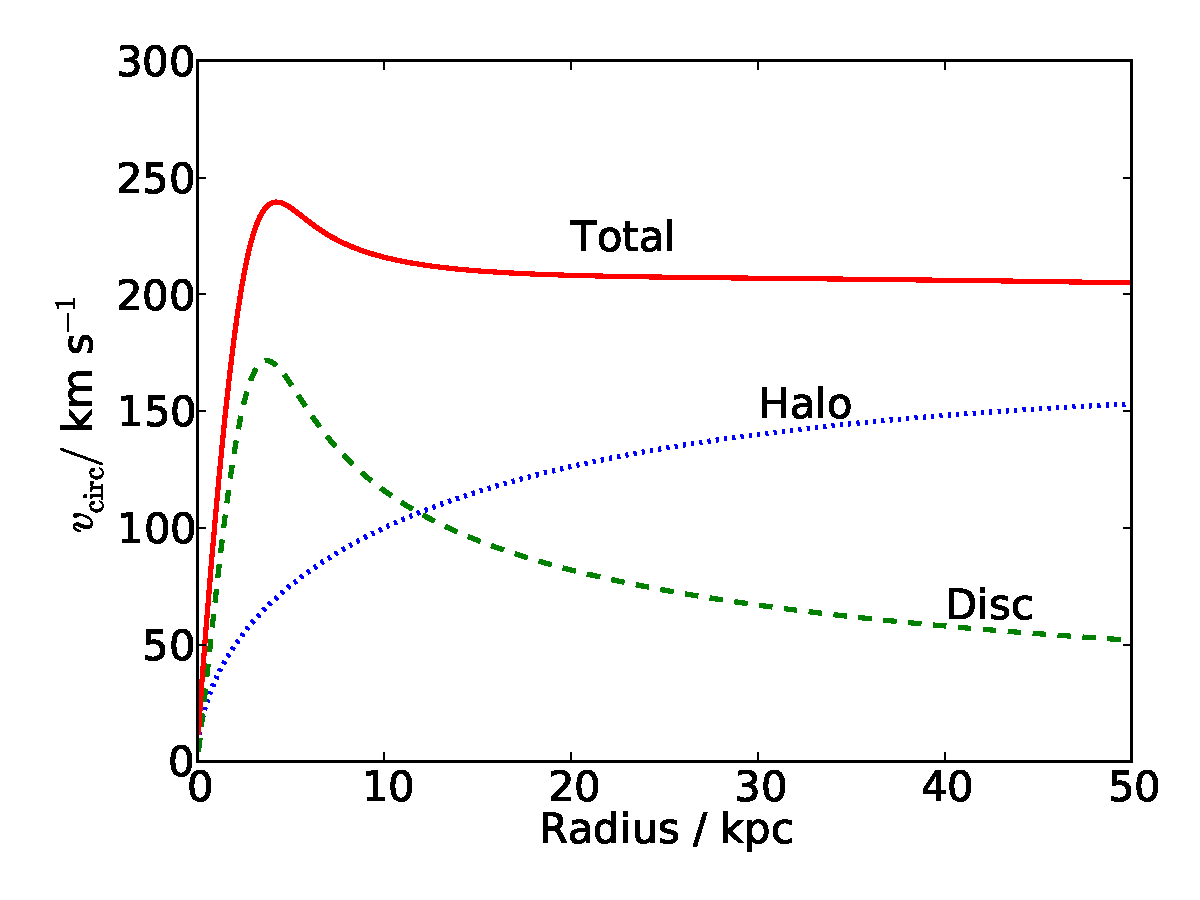
\includegraphics[width=0.8\textwidth]{RotationCurve.pdf}
  \caption[Schematic illustration of galaxy rotation curves]{Schematic illustration of galaxy rotation curves (circular velocity as a function of galactocentric distance). The contribution to the circular velocity from the luminous disc (green dashed line) and dark matter halo (red dotted line) are shown, as well as the total circular velocity (solid blue line). }
  \label{fig:intro:RotationCurves}
\end{figure}

We see that evidence for dark matter appears over a wide range of distance scales, from the cosmological horizon down to our own Milky Way. Dark matter is required to explain the formation and growth of large scale structure, the dynamics of both galaxies and galaxy clusters and the anisotropic temperature distribution of the CMB among others. In spite of this, there remain several problems and unanswered questions with the dark matter paradigm.


\todo{Need to talk about lensing observations...}
\todo{Nonbaryonic nature determined by primordial nucleosynthesis...}
\todo{Cite Lyndzo!}
\todo{Lensing?}
\todo{Tully-Fisher}
\todo{Bullet cluster}

\subsection{Problems with dark matter}

There have emerged several issues with the dark matter dominated model of structure formation as studied with N-body simulations. For example, DM-only simulations predict the existence of a large number of massive subhalos around Milky Way-size galaxies \cite{Springel:2008}. Using semi-analytical models of galaxy formation Kauffmann \etal \cite{Kauffmann:1993} predicted that a Milky Way-size halo should host over 100 subhalos massive enough to support observable satellite galaxies.  However, the known population of dwarf spheroidal (dSph) satellite galaxies for the Milky Way is on the order of 20 \cite{Walker:2009}, although more ultra-faint satellites are still being discovered (e.g. see Ref.~\cite{Belokurov:2010}). This discrepancy between the predicted and observed amount of substructure in CDM structure formation is often referred to as the `missing satellite problem' \cite{Klypin:1999}.

A related issue is the so-called `too big to fail' problem, which concerns the density of dark matter subhalos. In particular, it is found that the most massive DM subhalos found in N-body simulations are too massive to host the brightest of the Milky Way's dSph satellites \cite{Boylan-Kolchin:2011}. If the observed dSph galaxies are hosted instead by less massive subhalos, this leaves a large number of more massive DM halos which have not yet been accounted for \cite{Garrison-Kimmel:2014}. \note{NB: there are 11 well-known/bright/classical dSph satellites...}

Finally, there is also a discrepancy between the observed and simulated density profiles: the `Core-Cusp' problem (for a review, see Ref.~\cite{deBlok:2009}). Cosmological simulations indicate that the DM density should be sharply peaked near the centre of low surface brightness and dSph galaxies \cite{Dubinski:1991, Navarro:1996}. In contrast, observations of the rotation curves of a large number of galaxies suggests the presence of a core - a flat dark matter density profile near the centre \cite{Salucci:2001, Donato:2004}. While these results are still under contention (for example, Ref.~\cite{Hayashi:2004} find rotation curves consistent with \textit{cuspy} density profiles), they may indicate a significant difference between the process of structure formation in the universe and that extracted from \LCDM simulations.

A number of possible solutions to these issues have been suggested. Baryonic effects such as dynamical friction and stellar and supernova feedback (see for example Refs.~\cite{Gritschneder:2013, Amorisco:2014,DelPopolo:2014}) can lead to the expulsion of DM from the centres of subhalos, reducing the total halo mass and leading to a flatter central density profile. \note{This bit could be better.} Others have suggested that a \textit{warm} dark matter model may be a better fit to the data \cite{Moore:1999, Bode:2001, Maccio:2010}, reducing the amount of structure on small scales, as described in Sec.~\ref{intro:sec:properties}. \note{What about solutions about increasing the resolution of N-body simulations?} Whatever the ultimate resolution of these problems, it is clear that dark matter dominated structures such as dSph galaxies are testing ground for an even more precise understanding of structure formation in the DM paradigm.

There remains one problem which is of a much more theoretical nature. Dark matter is invoked to account for missing mass in a wide range of scenarios. However, this missing mass has not yet been observed indicating that it must interact only very weakly with photons and other particles of the standard model. In fact, as we shall see in Sec.~\ref{intro:sec:properties}, there is strong evidence that particles making up the universe's dark matter cannot be baryonic and must originate from beyond the Standard Model of particle physics. In the next section, we investigate what more can be inferred about the nature of particle dark matter and explore some well-motivated candidates.

\section{Properties of dark matter}
\label{intro:sec:properties}

Beyond its gravitational contribution to the universe, we appear to know little about the nature of particle dark matter. However, the success of modern cosmology and the lack of a confirmed detection so far means that we do have a grasp on some of the properties of any potential candidate. Taoso \etal \cite{Taoso:2008} present a `10-point test' which must be passed by any particle before it can be considered as a viable dark matter candidate. Here, I will briefly discuss four of these points, namely, that the DM candidate must be cold, neutral, produced with the appropriate relic density and compatible with primordial nucleosynthesis. \note{What about stability? THIS IS IMPORTANT FOR CANDIDATES - mention...}

\subsection{Coldness}

Results from N-body simulations indicate that dark matter should be \textit{cold}. That is, DM should be travelling non-relativistically when it decouples from the thermal bath in the early universe. \note{Not quite true - could be warm...} In practise, this typically means that it cannot be have a mass greater than around 1 keV \cite{Narayanan:2000}. \note{Watch out - this is actually the limit of WDM...}  The typical speed of DM particles in the early universe defines the so-called \textit{free-streaming length}. Below this length-scale, density perturbations are suppressed due to Landau damping \cite{Bond:1983}. For non-relativistic species, this free-streaming length scales as $m_\chi^{-1/2}$ for thermal relics of mass $m_\chi$ \cite{Boyanovsky:2008} \note{Why even say this...?}. For particle candidates which are too light - and which therefore travel too quickly after decoupling - small scale structures cannot form and cannot match the distribution of structures we see today. \note{Distinguish between warm and cold - what is the length scale?} \textit{Warm} dark matter candidates with keV-scale masses have been suggested to explain the subhalo structures at the scale of dSph galaxies (as has already been discussed) However, \textit{hot} dark matter, which decouples at relativistic speeds, is strongly-constrained and cannot make up more than around 1\% of the total dark matter component \cite{Abazajian:2005, dePutter:2012}.

\subsection{Neutrality}

\note{Include information about millicharged DM from notes!!!}


\subsection{Relic density}

\note{Include calculations from relic density notes at work!!!}


\subsection{Primordial nucleosynthesis}

\note{Need more refs here...}

Primordial nucleosynthesis (or Big Bang Nucleosynthesis, BBN) describes the production of light nuclei in the first few minutes after the big bang. By solving a set of coupled Boltzmann equations describing the nuclear reactions of protons, neutrons and light nuclei, we can obtain the primordial abundances of these light nuclei and compare with the inferred values. \note{Citation} Significantly, these abundances depend strongly on the baryon-photon ratio $\eta$ and therefore the total baryon density. Fits to data lead to the result $\Omega_b h^2 = 0.017 - 0.024$ \cite{Fields:2006}, independent of the value obtained from CMB measurements (Table~\ref{tab:intro:Planck}). Thus, the dark matter of the universe cannot be baryonic. \note{Combine this with the `neutrality' constraint and we see that there are no SM particles with the correct quantum numbers.} We are led to conclude that particle dark matter must consist of some as-yet undiscovered particle. \note{Link this to the next section...}

The results of BBN are also very sensitive to light new species, which can alter the number of relativistic degrees of freedom in the early universe and therefore affect the expansion rate. These include, for example, gravitinos \cite{Maggiore:2000}, right-handed neutrinos \cite{Cyburt:2005} and millicharged particles \cite{}. BBN therefore provides strong constraints on the parameters of such models. \note{What about stating some of the constraints on Nv?} In addition, the decay of dark matter particles into electromagnetic or hadronic showers during nucleosynthesis can drastically change the primordial abundances of the light elements. BBN can therefore be used to constrain models in which dark matter undergoes early decays (or in which dark matter is produced by the decays of heavier particles) \cite{Jedamzik:2006}.


\section{Particle dark matter candidates}
\label{intro:sec:candidates}

\note{arXiv:0903.4849}

Dark matter candidates can be found in a wide range of models of particle physics beyond the standard model.  \todo{This bit!}


The final condition appearing in the `10-point test' of Taoso \etal asks the question `Can it be probed experimentally?' While there are viable DM candidates which interact only gravitationally (such as the gravitino \note{need a ref}), a wide variety of proposed candidates can interact (however weakly) with the particles of the standard model. While the experimental accessibility of a given DM candidate is not a strict necessity, it allows models to be tested (and either falsified or confirmed) beyond the hypothesis stage. In the next section, we explore the different avenues by which models of particle dark matter may be probed.

\section{Detection of dark matter}

Many of the candidates which have been discussed are expected to interact weakly with the particles of the Standard Model. Dark matter particles which are produced by thermal freeze-out in the early universe must have interactions with SM \note{[Define SM somewhere]} particles in order to maintain thermal and kinetic equilibrium. These interactions are mediated by Feynman diagrams which can be represented (schematically) as in Fig.~\ref{intro:fig:diagrams}. The existence of production, annihilation and scattering processes between DM and SM particles provides a window into the possible detection of particle DM. Each of these processes leads to a distinct detection strategy, often referred to as collider, indirect and direction detection.

\begin{figure}[t]

	\centering
        \subbottom[Production]
                {\begin{fmffile}{DM1}
		\setlength{\unitlength}{0.08cm}
		\raisebox{0.2\height}{
                \begin{fmfgraph*}(40,25)
		\fmfleft{i1,i2}
		\fmfright{o1,o2}
		\fmf{fermion}{i1,v1}
		\fmf{fermion}{v1,o1}
		\fmf{fermion}{i2,v1}
		\fmf{fermion}{v1,o2}
		\fmflabel{$\psi$}{i1}
		\fmflabel{$\psi$}{i2}
		\fmflabel{$\chi$}{o1}
		\fmflabel{$\chi$}{o2}
		\fmfblob{.16w}{v1}
		\end{fmfgraph*}}
		\end{fmffile}\label{intro:fig:diagramsa}}
        \subbottom[Annihilation]
                {\begin{fmffile}{DM2}
		\setlength{\unitlength}{0.08cm}
                \raisebox{0.2\height}{
		\begin{fmfgraph*}(40,25)
		\fmfleft{i1,i2}
		\fmfright{o1,o2}
		\fmf{fermion}{i1,v1}
		\fmf{fermion}{v1,o1}
		\fmf{fermion}{i2,v1}
		\fmf{fermion}{v1,o2}
		\fmflabel{$\chi$}{i1}
		\fmflabel{$\chi$}{i2}
		\fmflabel{$\psi$}{o1}
		\fmflabel{$\psi$}{o2}
		\fmfblob{.16w}{v1}
		\end{fmfgraph*}}
		\end{fmffile}\label{intro:fig:diagramsb}}
         \subbottom[Scattering]
                {\begin{fmffile}{DM3}
		\setlength{\unitlength}{0.08cm}
                \raisebox{0.2\height}{
		\begin{fmfgraph*}(40,25)
		\fmfleft{i1,i2}
		\fmfright{o1,o2}
		\fmf{fermion}{i1,v1}
		\fmf{fermion}{v1,o1}
		\fmf{fermion}{i2,v1}
		\fmf{fermion}{v1,o2}
		\fmflabel{$\psi$}{i1}
		\fmflabel{$\chi$}{i2}
		\fmflabel{$\psi$}{o1}
		\fmflabel{$\chi$}{o2}
		\fmfblob{.16w}{v1}
		\end{fmfgraph*}}
		\end{fmffile}\label{intro:fig:diagramsc}}
   \caption[Schematic dark matter interactions]{Schematic interactions between dark matter particles $\chi$ and standard model particles $\psi$.}
\label{intro:fig:diagrams}
\end{figure}

\subsection{Collider production}

\subsection{Indirect detection}

The possibility of dark matter annihilation into SM particles (as described in Fig.~\ref{intro:fig:diagramsb}) means that DM may be detected indirectly, by searching for these excess annihilation products. A number of experiments may be sensitive to such signals which may be in the form of 

These annihilation products may be in the form of 

In pratice, such searches are most effective when 

POSITRONS (PAMELA \cite{Boezio:2009} and AMS \cite{Aguilar:2013})

NEUTRINOS (ANTARES/KM3NeT and ICECUBE \cite{Aartsen:2013b} -I'll talk more about that in the later chapters)

FERMI-LAT (Collaboration) \cite{Ackerman:2012}

GAMMA RAYS (1-3 GeV, 130 GeV [original Weniger paper \cite{Weniger:2012}], general limits from dSph and galaxy)

ICECUBE SEARCHES FOR DM ANNIHILATION IN GALAXIES AND CLUSTERS \cite{Aartsen:2013}

IACTS: HESS, MAGIC, VERITAS and CTA \cite{Doro:2013}

Another promising source of 

\todo{Arrange by 1) signal that's being looked for (and therefore which experiment is looking for it) OR 2) where experiments are looking...maybe the second option makes more sense...}

\subsection{Direct detection}

Processes described by the diagram in Fig.~\ref{intro:fig:diagramsc} lead to the possibility of scattering between DM and SM particles. The principle of direct detection is to look for nuclear recoils due to this scattering in a dedicated detector \cite{Goodman,Drukier}. However, WIMPs with GeV-scale masses and speeds $v \sim 10^{-3} c$ (as predicted by N-body simulations \cite{Diemand} and direct calculations \cite{}) are expected to produce keV-scale nuclear recoils. In addition, due to the expected low cross section for such interactions, the predicted rate is less than around 1 event per year per kg of detector mass \note{Check and cite}. Detecting such rare, low energy recoils requires not only large ton-scale detectors, but also sophisticated methods for discriminating signal from background.



